\documentclass[12pt,a4paper]{article}
\usepackage[T2A]{fontenc}
\usepackage[utf8]{inputenc}
\usepackage[russian]{babel}
\usepackage{amsmath}
\usepackage{amssymb}
\usepackage{graphicx}
\usepackage{floatrow}
\usepackage{booktabs}
%\usepackage{wrapfig}
\usepackage{lipsum}
%\usepackage{subcaption}
\usepackage{fancyhdr}


%multi-column
%\multicolumn{number cols}{align}{text} % align: l,c,r

%multi-row
\usepackage{multirow}

\newcommand{\figref}[1]{(См. рис. \ref{#1})}
\newcommand{\secref}[1]{(См. раздел. \ref{#1})}

\newcommand{\e}[1]{\text{$\cdot10^{#1}$}}

\pagestyle{fancy}
\fancyhead{}
\fancyhead[L]{Работа 5.8.1}
\fancyhead[R]{}
\fancyfoot[C]{\thepage}

\renewcommand{\cot}{\text{ctg}}

\author{\normalsize Маслов Артем, Дедков Денис \\
	\normalsize группа Б01-108 \\
	\normalsize 01.10.2022}
\date{}

\usepackage{float}
\restylefloat{table}
\title{
	\large Отчет о выполнении лабораторной работы 3.6.1 \\
	\Large Спектральный анализ электрических сигналов \\ 
	
}

\begin{document}
\maketitle
\subsection*{} В работе изучен...

\subsection*{Оборудование и приборы} Генератор сигналов специальной формы
АКИП-3409/4, Цифровой осциллограф SIGLENT АКИП 4131/1.

\subsection*{Введение}

\subsection*{Ход работы}

\subsubsection*{Калибровка оптического пирометра}

Для калибровки шкалы приборов было проведено сравнение показаний пирометра с показаниями термопары модели АЧТ. 

Постоянная термопары была получена из графика, приведенного в лабораторной работе:
$$\Psi = (39 \pm 1) \text{ мкВ/дел.}$$

Для уменьшения случайной погрешности, мы провели целую серию измерений. В таблице приведены полученные значения. Сравнение случайной ошибки ($\sim0.5^\circ C$) с ошибкой пирометра в данном диапазоне температур ($\sim10^\circ C$) позволяет не учитывать её при расчете погрешностей. Оценка ошибки измерения термопары можно оценить суммой случайной погрешности ($\sim0.015\;\text{мкВ}$) и ошибки округления ($\sim0.005\;\text{мкВ}$). Однако основную неточность в измерении финальной температуры вносит неизвестная температура комнаты. Относительная погрешность вычисленной температурой будет совпадать с относительной ошибкой измерения напряжения. 

\begin{table}[H]
	\addtolength{\tabcolsep}{-4pt}
	\footnotesize
	\begin{tabular}{ccc}
\toprule
$T_{p}, ^oC$ & $V$, мВ & $T_{t}, ^oC$ \\
\midrule
947.0 & 36.4 & 936.5 \\
937.0 & 36.4 & 935.0 \\
939.0 & 36.3 & 934.5 \\
939.0 & 36.3 & 933.5 \\
938.0 & 36.3 & 933.5 \\
938.0 & 36.3 & 933.5 \\
938.0 & 36.3 & 933.3 \\
937.0 & 36.3 & 932.5 \\
939.0 & 36.3 & 932.5 \\
938.0 & 36.3 & 932.5 \\
\bottomrule
\end{tabular}

	\begin{tabular}{cccc}
\toprule
$T, ^oC$ & $I$, А & $V$, В & $W$, Вт \\
\midrule
963.0 & 0.56 & 2.12 & 1.19 \\
1102.0 & 0.59 & 2.39 & 1.41 \\
1057.0 & 0.57 & 2.19 & 1.25 \\
1198.0 & 0.64 & 2.88 & 1.84 \\
1288.0 & 0.69 & 3.40 & 2.33 \\
1424.0 & 0.75 & 4.17 & 3.13 \\
1556.0 & 0.84 & 5.22 & 4.37 \\
1750.0 & 0.99 & 7.36 & 7.30 \\
1897.0 & 1.10 & 8.95 & 9.83 \\
\bottomrule
\end{tabular}

	\caption{Проверка закона Стефана-Больцмана. Эксперимент по нагреванию вольфрамовой нити..}
\end{table}

Выражения, полученные для температур, измеренных термопарой ($T_t$) и пирометром  ($T_p$) соответственно:

$$T_t = (934 \pm 5)\;^oC,\;\; T_p = (939 \pm 12)\;^oC.$$

Выражения для температур отлично согласуются в пределах ошибок измерений.

\subsubsection*{Проверка закона Стефана-Больцмана}

Для проверки выполнения закона Стефана-Больцмана, проведена обработка данных эксперимента по нагреву вольфрамовой нити лампы накаливания. Собранные данные приведены в таблице.


Измеренная яркостная температура преобразуется в термодинамическую температуру с помощью графика зависимости $T(T_{\text{ярк}})$. Мощность, потребляемая лампой, легко оценивается с использованием закона Джоуля-Ленца: $W = UI$. Эта мощность равна рассеянной по закона сохранения энергии. График зависимости рассеиваемой мощности от температуры приведена на рисунке \ref{fig:linwt}.

\begin{figure}[h]
	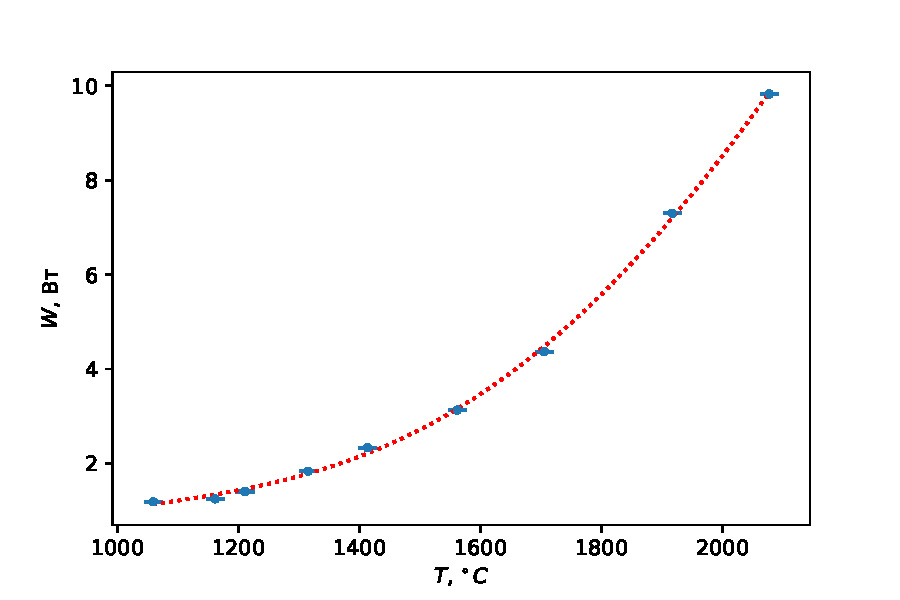
\includegraphics[scale=0.8]{gen/fig-wt.pdf}
	\caption{Зависимость $W(T)$.}
	\label{fig:wt}
\end{figure}

Для точного вычисления степени в законе Стефана-Больцмана, проведем линеаризацию зависимости $W(T)$: 

$$\ln W = \ln (\varepsilon_T S \sigma) + n \ln T. $$

График получившейся зависимости изображен на рисунке \ref{fig:linwt}. Подсчет коэффициентов проведем методом наименьших квадратов (МНК):


\begin{figure}[h!]
	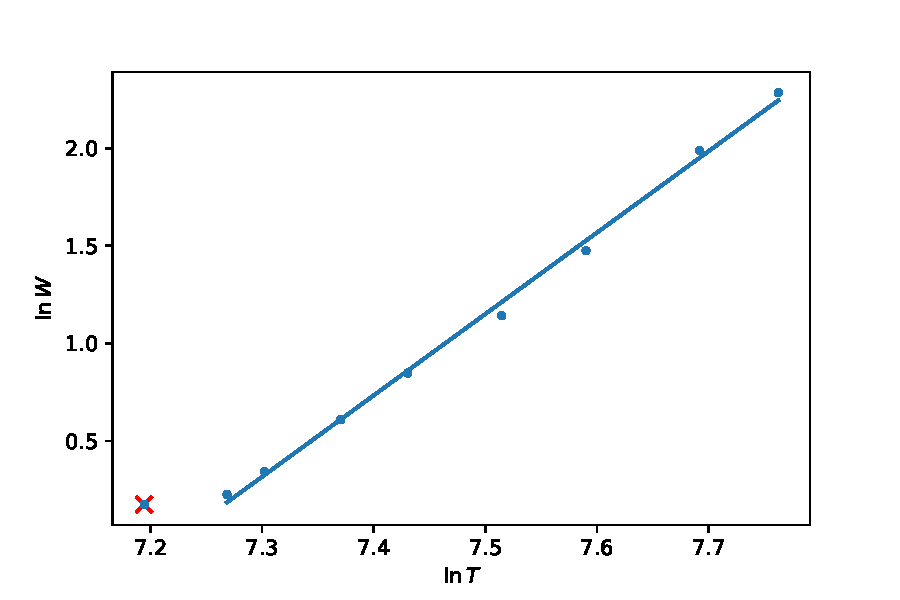
\includegraphics[scale=0.8]{gen/fig-linwt.pdf}
	\caption{Зависимость $\ln W ( \ln T).$}
	\label{fig:linwt}
\end{figure}

\begin{table}[H]
	\addtolength{\tabcolsep}{-4pt}
	\footnotesize
	\begin{tabular}{ccccccccc}
\toprule
$\overline{x}$ & $\sigma_x^2$ & $\overline{y}$ & $\sigma_y^2$ & $r_{xy}$ & $a$ & $\Delta a$ & $b$ & $\Delta b$ \\
\midrule
7.46e+00 & 3.40e-02 & 1.01e+00 & 5.29e-01 & 1.33e-01 & 3.92 & 0.18 & -28.20 & 1.37 \\
\bottomrule
\end{tabular}

	\caption{Статистическая обработка зависимости $\ln W ( \ln T).$}
\end{table}

Тогда финальное выражение для степени в законе Стефана-Больцмана:
$$n = (3.92 \pm 0.18).$$


\subsubsection*{Оценка коэффициента Стефана-Больцмана}

Для оценки коэффициента Стефана-Больцмана, нужно учесть тот факт, что вольфрамовая нить черным телом не является. А значит, следует уточнить закон Стефана-Больцмана множителем серого тела $\varepsilon_T$.
В ней же приведена зависимость коэффициента ослабления $\varepsilon_T$ для вольфрама.

Коэффициента Стефана-Больцмана легко рассчитать по следующей формуле:
$$\sigma = \frac{W}{\varepsilon_T(T) \cdot S \cdot T^4}$$
 
Погрешность же, по правилам оценки погрешностей косвенных вычислений, можно оценить суммой относительных ошибок каждой величины:
$$\delta_\sigma \approx \sqrt{\epsilon_S^2 + (4\epsilon_T)^2}$$

График с крестами погрешностей показан на рисунке \ref{fig:sigma}. Видно, что при увеличении температуры, коэффициент Стефана-Больцмана уменьшается.

\begin{figure}[h]
	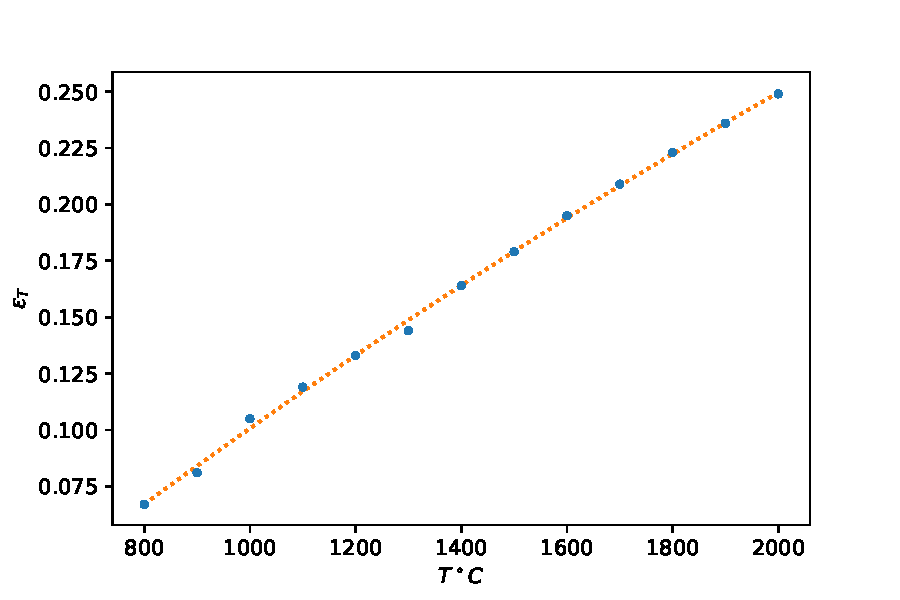
\includegraphics[scale=1.2, width=0.47\linewidth]{gen/fig-epsilon.pdf}\hfill
	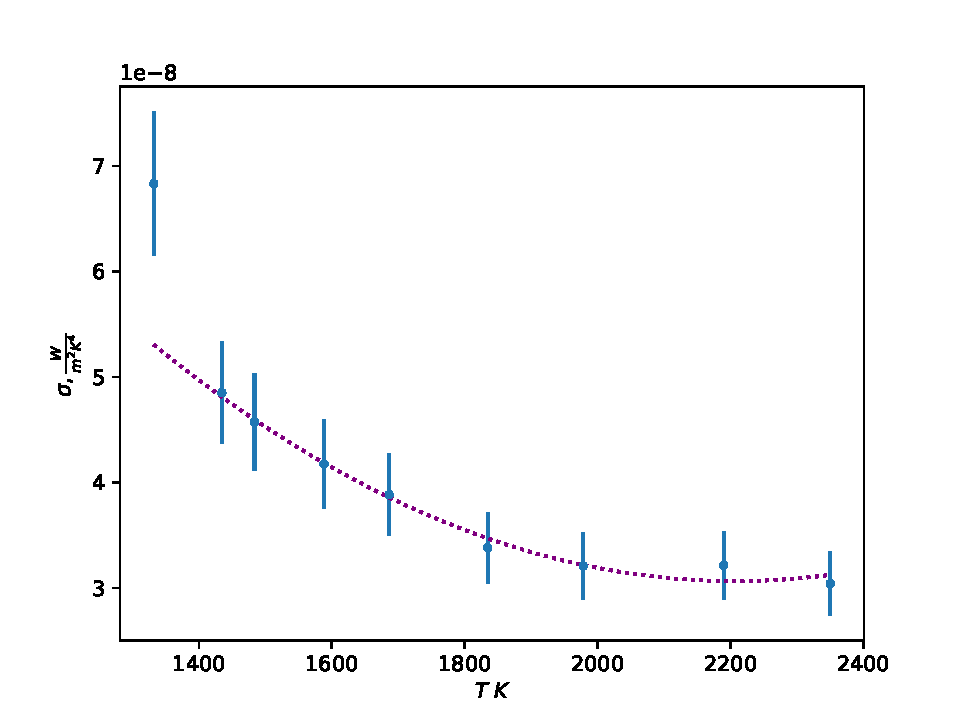
\includegraphics[scale=1.2, width=0.47\linewidth]{gen/fig-sigma.pdf}
	\caption{Зависимость $\ln W ( \ln T).$}
	\label{fig:sigma}
\end{figure}

\subsection*{Вывод}

В работе была проверена калибровка оптического пирометра путем сравнения измеренной температуры АЧТ с показаниями термопары. Показания термопары ($T_p$) и пирометра ($T_p$) хорошо согласуются:

$$T_t = (934 \pm 5)\;^oC,\;\; T_p = (939 \pm 12)\;^oC.$$

Был экспериментально вычислен показатель степени в законе Стефана-Больцмана. В пределах точности эксперимента $n$ сходится с теоретическим значением:
$$n = (3.92 \pm 0.18).$$

Также были вычислены коэффициенты $\sigma$ при различных температурах. Значения по порядку сходятся с эталонным значением. Также приведен график зависимости $\sigma$ от температуры (см. рис. \ref{fig:sigma}).

	
\end{document}